\documentclass[11pt]{article}
\usepackage[letterpaper,margin=1in]{geometry}
\usepackage[T1]{fontenc}
\usepackage{lmodern,microtype}
\usepackage{amsmath,amssymb,amsthm}
\usepackage{booktabs,tabularx,array,graphicx}
\usepackage{tikz}
\usetikzlibrary{arrows.meta,positioning}
\usepackage[numbers,sort&compress]{natbib}
\usepackage[colorlinks=true,linkcolor=black,citecolor=black,urlcolor=blue]{hyperref}

% ---------------------------------------------------------------------------
% Authorship is intentionally left blank.
% ---------------------------------------------------------------------------
\newcommand{\PaperAuthor}{}
\newcommand{\PaperAffiliation}{}

\hypersetup{
  pdftitle={When can a negative recovery assay exclude a recoverable subpopulation?},
  pdfsubject={Sharp coverage, stage-mismatch and allocation bounds for paired recovery observations},
  pdfkeywords={recovery assay, partial identification, negative observations,
               minimax design, finite-sample certificate, formal verification}}

\newtheorem{theorem}{Theorem}[section]
\newtheorem{proposition}[theorem]{Proposition}
\newtheorem{corollary}[theorem]{Corollary}
\newtheorem{lemma}[theorem]{Lemma}
\theoremstyle{definition}
\newtheorem{example}[theorem]{Example}
\theoremstyle{remark}
\newtheorem{remark}[theorem]{Remark}

\newcommand{\E}{\mathbb{E}}
\newcommand{\Prob}{\mathbb{P}}
\newcommand{\Rfull}{R_{\mathrm{full}}}
\newcommand{\hc}{h(c)}
\newcommand{\leanref}[1]{\texttt{#1}}
\newcolumntype{Y}{>{\raggedright\arraybackslash}X}
\setlength{\emergencystretch}{2em}

\newcommand{\planningrows}{%
$c=1$, $d=.5$ & 0.187500000 & 1597 & 1598 & 0.0498338\\
$c=.95$, $d=.5$ & 0.163125000 & 1835 & 1836 & 0.0499157\\
Also $\kappa=.90$, $\eta=.05$ & 0.139471875 & 2147 & 2148 & 0.0498894\\
Also $\delta=.01$ & 0.139471875 & 2300 & 2300 & 0.0499494\\
\midrule
Full range, $c=1.5$, $d=.5$ & 0.427500000 & 749 & 750 & 0.0498285\\
}


\title{When can a negative recovery assay exclude a recoverable
subpopulation?\\[4pt]
\large Sharp coverage, stage mismatch and allocation bounds for paired
observations}
\author{\PaperAuthor}
\date{17 September 2026}

\begin{document}
\maketitle

\begin{abstract}
A finite recovery experiment that records no qualifying event is compatible both
with the absence of recoverable units and with a failure to observe their
recovery. We give a sharp conditional separation of the two explanations for a
gated two-stage source observed under two alternative conditions, with
activation and subsequent progeny probabilities $(x,y)$ and $(a,b)$. If the two
conditions cover each stage, $x+a\ge c$ and $y+b\ge c$, and the within-condition
stage mismatch obeys $|x-y|\le d$, the equally weighted complete-path response
is at least $\Rfull(c,d)=\bigl(c^2-t^2\bigr)/4$ with $t=\min\{d,\min(c,2-c)\}$,
and this is attained. Because $c$ bounds a sum of two probabilities, its range
is $[0,2]$; on the restricted range $c\le1$ the bound reduces to
$\max\{0,c^2-d^2\}/4$, and for $c>1$ a positive floor of at least $c-1$ holds
with no mismatch information at all. We compute the exact worst-case response of
every fixed allocation weight $w$, which has three regimes, is maximized at
$w=1/2$, and is strictly suboptimal away from $w=1/2$ exactly when the mismatch
budget binds. The uniform mismatch bound can be weakened to a mean-square budget
$\E[(x-y)^2]\le D^2$ without changing the floor. With conditional recording
probability at least $\kappa$ on a covered fraction $1-\eta$ of recoverable
types, the usable floor is $g=(1-\eta)\kappa\Rfull(c,D)$. For an even number $n$
of independent eligible units split equally between the two conditions, and
recoverable fraction at least $\theta$, the worst-case all-negative probability
is exactly $(1-\theta g)^n$; a conditional calibration-failure allowance $\delta$
gives the sharp total bound $\delta+(1-\delta)(1-\theta g)^n$. A finite balanced
design achieves total error $\alpha$ if and only if $\theta g>0$ and
$\delta<\alpha$, or $\theta g=1$ and $\delta\le\alpha$; no history-dependent
reallocation of the same budget improves the guarantee. The coverage, allocation,
mean-square, population and decision inequalities are verified in Lean~4. A
synthetic example needs $2{,}300$ units to exclude a recoverable fraction of one
per cent at five per cent error under its declared premises, and $750$ units when
the coverage assumptions are strengthened beyond the restricted range. The result
identifies a joint calibration requirement; it does not validate any particular
assay, and non-detection is not evidence of irreversible death.
\end{abstract}

\section{The question answered by a negative record}\label{sec:intro}

Failure to observe progeny after an exposure is consistent with several
explanations: there were no recoverable units; recovery was delayed past the
observation deadline; activation occurred but reproduction did not qualify;
units were lost in handling; or the instrument failed to record a genuine event.
These explanations support very different decisions. Statistical regrowth assays
and the minimum-duration-for-killing framework are established tools for
quantifying tolerance \citep{brauner2016,brauner2017}, individual-level recovery
has been followed since the phenotypic-switch experiments of
\citet{balaban2004}, and the vocabulary of resistance, tolerance and persistence
has agreed definitions \citep{balaban2019}. We do not propose new biological
definitions. Our question is narrower and quantitative:

\begin{quote}
Under which explicit, checkable recovery assumptions does an all-negative finite
experiment exclude a recoverable fraction of at least $\theta$, and how many
units does that take?
\end{quote}

Without a restriction connecting recoverability to a finite observation, no
uniform answer exists. If a recoverable fraction $p$ has conditional
detection-time distribution $F$, the observable cumulative event probability
through the deadline $T$ is $r(t)=pF(t)$; for every $p'\ge r(T)$ one may set
$F'=r/p'$ on $[0,T]$ and place the remaining mass after $T$, reproducing the
record exactly. This is the elementary form of a familiar obstruction in
censored-event and cure-fraction models \citep{maller1992,amico2018}, and is a
partial-identification statement in the sense of \citet{manski2003}. It is also
why the classical zero-numerator devices \citep{hanley1983,clopper1934,tuyl2009}
answer a different question: the rule of three bounds a \emph{detectable} event
rate, not a latent recoverable fraction, and the gap between the two is exactly
what must be assumed or calibrated. The viable-but-nonculturable literature
\citep{oliver2010} is a standing reminder that the gap can be large.

The restriction studied here concerns two serial stages and two alternative
observation conditions. It is not enough for the two conditions to cover each
stage somewhere: the source state $(x,y,a,b)=(1,0,0,1)$ has full first-stage
coverage in condition~1 and full second-stage coverage in condition~2, yet
neither condition completes a path, so no number of units observed under these
conditions can detect it. We quantify the additional connection required. The
cross-condition coverage level $c$ must exceed the within-condition stage
mismatch $d$, and the resulting floor composes with recording losses, hidden
types, a fixed balanced design and a calibration allowance into an explicit
finite sample size.

\subsection{Contributions}

\begin{enumerate}
\item \textbf{A sharp coverage floor on the full parameter range}
(Theorem~\ref{thm:coverage}). Since $c$ bounds the sum of two probabilities, the
natural range is $0\le c\le2$. The sharp equally weighted complete-path floor is
$\Rfull(c,d)=(c^2-t^2)/4$ with $t=\min\{d,\hc\}$ and $\hc=\min(c,2-c)$. On
$c\le1$ this is the positive-part formula $\max\{0,c^2-d^2\}/4$; for $c>1$ it is
at least $c-1$ \emph{with no mismatch hypothesis}
(Corollary~\ref{cor:highcov}). The frequently quoted ceiling of $1/4$ for such
floors is an artefact of the restricted range, not a limit on paired recovery
sensitivity.
\item \textbf{The exact allocation profile} (Theorem~\ref{thm:profile}). For
every allocation weight $w\in[0,1]$ we compute the exact worst-case response,
which has three regimes in $A=|2w-1|$. Equal allocation is maximin; it is the
\emph{unique} maximin allocation exactly when the mismatch budget binds
($t<\hc$), and otherwise the optimum is a plateau of width $\hc/c$ in $A$
(Corollaries~\ref{cor:strict} and~\ref{cor:plateau}). This replaces a numerical
grid search, which cannot distinguish a plateau from a flat numerical optimum.
\item \textbf{Mismatch in mean square} (Theorem~\ref{thm:moment}). The uniform
per-type bound $|x_z-y_z|\le d$ may be replaced by the population budget
$\E[(x-y)^2]\le D^2$ without changing the floor, which is again $\Rfull(c,D)$
and again attained. The uniform bound is the special case $D=d$. We also show
which pooled summaries are \emph{not} sufficient: equal stage means permit a
zero floor, and the pooled second-stage conditional probability is
$\E[xy]/\E[x]$, not $\E[y]$ (Examples~\ref{ex:means} and~\ref{ex:pooled}).
\item \textbf{An exact finite decision rule} (Theorem~\ref{thm:root} and
Section~\ref{sec:sample}). The all-negative certificate has worst-case error
exactly $\delta+(1-\delta)(1-\theta g)^n$ with $g=(1-\eta)\kappa\Rfull(c,D)$,
the likelihood being derived from the source paths rather than postulated. A
finite balanced design suffices if and only if $\theta g>0$ and $\delta<\alpha$,
or $\theta g=1$ and $\delta\le\alpha$ (Theorem~\ref{thm:feasible}); the second
regime exists only because the coverage range was extended.
\item \textbf{No gain from adaptive reallocation} (Theorem~\ref{thm:adaptive}).
On the least detectable source both conditions respond identically, so every
history-dependent allocation policy with the same budget and the same qualifying
event faces the same bound.
\item \textbf{Machine-checked core.} The coverage bound and its witnesses, the
allocation profile and its witnesses, the mean-square population floor, the
balanced sampling identity and inequality, the calibration composition, and the
feasibility characterization are verified in Lean~4 \citep{moura2021} against a
pinned Mathlib \citep{mathlib2020}. Section~\ref{sec:formal} states exactly which
results are compiled and which are conventional.
\end{enumerate}

The mathematical ingredients are elementary: polynomial inequalities on a
rectangle, finite probability sums, and a monotone one-dimensional optimisation.
The contribution is the sharp, explicit and composable route from a source
assumption to a finite decision, together with a precise account of what such a
decision cannot do. In particular, nothing here licenses the inference that a
unit which fails to recover by $T$ is dead.

\section{Target, source events and sampling units}\label{sec:model}

Fix an exposure duration $\tau$ and a separate recovery-observation deadline
$T$; these are different experimental clocks. Fix an intermediate activation
time $t_A<T$ and a prespecified \emph{reference task} that defines
recoverability independently of whether the test conditions detect a unit by
$T$. Let $p\in[0,1]$ denote the fraction of reference-recoverable units in the
population from which eligible units are sampled independently. A unit may be a
cell, a cluster or a lineage; its meaning, sampling scheme and denominator must
be fixed before $p$ is interpreted.

For a recoverable latent type $z$, let $A_j$ be activation by $t_A$ and $D_j$ the
specified qualifying progeny event by $T$, in condition $j\in\{1,2\}$, and write
\begin{equation}\label{eq:stages}
x_z=\Prob(A_1\mid z),\quad y_z=\Prob(D_1\mid A_1,z),\quad
a_z=\Prob(A_2\mid z),\quad b_z=\Prob(D_2\mid A_2,z).
\end{equation}
By the chain rule the complete early-activation paths have probabilities
$x_zy_z$ and $a_zb_z$; no independence between the stages is assumed. If the
instrument also records qualifying paths with later activation, these two paths
are sufficient subevents of the positive event, and the lower bounds below
remain valid. When an activation probability is zero, the corresponding
second-stage parameter is an off-path source parameter: it cannot be estimated by
conditioning on observations that never occur, and any constraint involving it
is structural or counterfactual rather than an observed conditional frequency.

Figure~\ref{fig:paths} shows the terminal source events; Table~\ref{tab:symbols}
fixes the symbols and their domains.

\begin{figure}[ht]
\centering
\resizebox{\linewidth}{!}{%
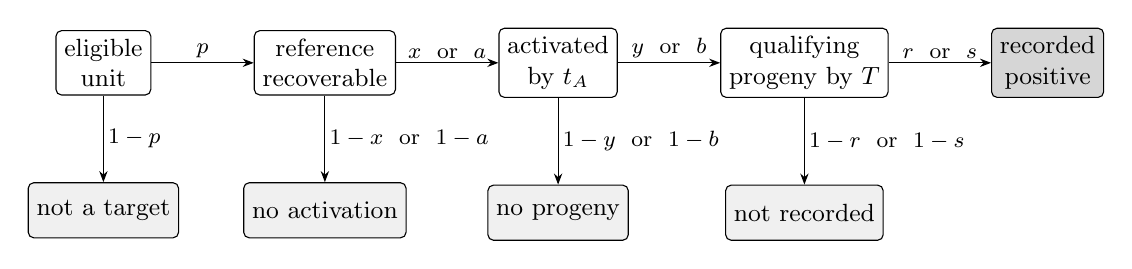
\begin{tikzpicture}[>={Stealth[length=4pt]},node distance=11mm and 13mm,
  every node/.style={font=\small},
  box/.style={draw,rounded corners=2pt,minimum height=7mm,
    align=center,inner sep=3pt},
  miss/.style={box,fill=black!6},
  hit/.style={box,fill=black!16},
  lab/.style={font=\footnotesize,inner sep=1.5pt}]
\node[box] (elig) {eligible\\unit};
\node[box,right=of elig] (rec) {reference\\recoverable};
\node[box,right=of rec] (act) {activated\\by $t_A$};
\node[box,right=of act] (prog) {qualifying\\progeny by $T$};
\node[hit,right=of prog] (obs) {recorded\\positive};
\node[miss,below=of elig] (n1) {not a target};
\node[miss,below=of rec] (n2) {no activation};
\node[miss,below=of act] (n3) {no progeny};
\node[miss,below=of prog] (n4) {not recorded};
\draw[->] (elig) -- node[lab,above] {$p$} (rec);
\draw[->] (rec) -- node[lab,above] {$x$ \ or \ $a$} (act);
\draw[->] (act) -- node[lab,above] {$y$ \ or \ $b$} (prog);
\draw[->] (prog) -- node[lab,above] {$r$ \ or \ $s$} (obs);
\draw[->] (elig) -- node[lab,right] {$1-p$} (n1);
\draw[->] (rec) -- node[lab,right] {$1-x$ \ or \ $1-a$} (n2);
\draw[->] (act) -- node[lab,right] {$1-y$ \ or \ $1-b$} (n3);
\draw[->] (prog) -- node[lab,right] {$1-r$ \ or \ $1-s$} (n4);
\end{tikzpicture}}
\caption{Terminal source events for one unit. Arrow labels are conditional
probabilities for a fixed recoverable type: the first entry of each pair applies
in condition~1 and the second in condition~2, so the two conditions differ only
in which pair of stage probabilities governs the two gates. The four shaded
states on the bottom row all produce a negative record, as does an unrecorded
completed path. Failure at a gate contributes to the negative record but does not
imply irreversible incapacity. The recording probabilities $r$ and $s$ are
conditional on the completed path and the type.}
\label{fig:paths}
\end{figure}

\begin{table}[ht]
\centering\small
\begin{tabularx}{\linewidth}{@{}l l Y@{}}
\toprule
Symbol & Domain & Meaning\\
\midrule
$p,\theta$ & $p\in[0,1]$, $0<\theta\le1$ & Recoverable fraction and exclusion threshold\\
$x,y,a,b$ & $[0,1]$ & Conditional stage probabilities of a recoverable type\\
$c$ & $[0,2]$ & Cross-condition stage-coverage lower bound\\
$d,D$ & $[0,1]$ & Uniform and mean-square within-condition mismatch bounds\\
$\hc,t$ & $\hc=\min(c,2-c)$, $t=\min(d,\hc)$ & Attainable stage width and the binding mismatch\\
$\kappa,\eta$ & $[0,1]$ & Conditional recording floor and exceptional recoverable mass\\
$\delta,\alpha$ & $0\le\delta<\alpha<1$ & Calibration-failure allowance and total error budget\\
$n=2m$ & $m\ge1$ integer & Independent eligible units, allocated equally\\
$g$ & $[0,1]$ & Average recorded detection floor among recoverable units\\
\bottomrule
\end{tabularx}
\caption{Symbols and domains. The floor $g$ is neither an instrumental accuracy
score nor a lower bound on $p$. The coverage level $c$ bounds a \emph{sum} of two
probabilities, which is why its range is $[0,2]$.}
\label{tab:symbols}
\end{table}

Type populations are finite, with weights $\mu_z\ge0$ and $\sum_z\mu_z=1$
\emph{conditional on reference recoverability}. The same population supplies both
groups, and assignment is independent of latent type; randomly assigning
independent units to two fixed-size groups is one realization. Sorted
subpopulations, repeated images of one unit, related descendants of one founder
and sampling without replacement from a fixed specimen are \emph{not} this
model. Non-target units do not generate a positive in the exact source law;
background events that only add positives preserve the one-sided negative-record
bound, although reading a positive as proof of the target would require a
separate specificity argument.

\section{Why a finite negative record alone decides nothing}\label{sec:obstruction}

We record the three obstructions that motivate the source restriction. They are
elementary and are stated to fix the scope of the later results, not claimed as
new.

\begin{proposition}[Finite-follow-up identified set]\label{prop:ident}
Suppose the conditional detection-time distribution among recoverable units is
$F$ and the observable cumulative event probability is $r(t)=pF(t)$ for
$0\le t\le T$. Then the set of recoverable fractions compatible with exact
knowledge of $r$ on $[0,T]$, with no restriction on the distribution after $T$,
is $[r(T),1]$.
\end{proposition}

\begin{proof}
Any compatible $p'$ satisfies $p'\ge p'F(T)=r(T)$. Conversely, for $p'\in(0,1]$
with $p'\ge r(T)$ put $F'(t)=r(t)/p'$ on $[0,T]$, which is nondecreasing with
$F'(T)=r(T)/p'\le1$, and place the remaining mass $1-F'(T)$ after $T$. Then
$p'F'=r$ on $[0,T]$. If $r(T)=0$ the explanation $p'=0$ also fits, with any $F'$.
\end{proof}

An all-negative finite sample carries sampling uncertainty \emph{in addition} to
this structural ambiguity; more precise measurement of the same finite event law
does not shrink the identified set.

\begin{proposition}[Successful-only timing is uninformative for the
denominator]\label{prop:timing}
Among events detected by $T$, the timing distribution is $F(t)/F(T)$. For any
$\lambda\in(0,1]$, replacing $F$ by $\lambda F$ on $[0,T]$ and moving the removed
mass after $T$ leaves $F(t)/F(T)$ unchanged while multiplying the total detection
probability by $\lambda$.
\end{proposition}

Selected resuscitation analyses normalize by observed recovery events and study
their timing and trajectories \citep{fang2023}. Such data inform recovery
dynamics and motivate separating the stages, but by Proposition~\ref{prop:timing}
they do not by themselves calibrate the unseen recoverable mass or the paired
coverage used below.

\begin{example}[The serial-path obstruction]\label{ex:obstruction}
Let $(x,y,a,b)=(1,0,0,1)$. Then $x+a=y+b=1$, so each stage is covered by one of
the two conditions, yet $xy=ab=0$: neither condition completes a path. Every unit
of this type is negative in both conditions with probability one, so no number of
units observed under these conditions can detect it. Stage-wise coverage and
complete-path coverage are different quantities, and the mismatch $|x-y|=1$ is
what separates them.
\end{example}

\section{The sharp coverage floor}\label{sec:coverage}

Throughout this section, fix $0\le c\le2$ and $d\ge0$ and consider the source set
\begin{equation}\label{eq:adm}
\mathcal A(c,d)=\bigl\{(x,y,a,b)\in[0,1]^4:\ x+a\ge c,\ y+b\ge c,\ |x-y|\le
d\bigr\}.
\end{equation}
The description is asymmetric: coverage is required of both stages across the two
conditions, while mismatch is controlled within condition~1. Relabelling the
conditions is permitted only with a correspondingly justified mismatch bound.
Exact complementarity, $a=1-x$ and $b=1-y$, is \emph{not} assumed; it is the
special case treated in Corollary~\ref{cor:approx}. Write
\begin{equation}\label{eq:hrange}
\hc=\min(c,2-c),\qquad t=\min\{d,\hc\},\qquad
\Rfull(c,d)=\frac{c^2-t^2}{4}.
\end{equation}

\begin{theorem}[Sharp coverage floor]\label{thm:coverage}
For $0\le c\le2$ and $d\ge0$,
\[
\min_{(x,y,a,b)\in\mathcal A(c,d)}\frac{xy+ab}{2}=\Rfull(c,d),
\]
and the minimum is attained at
\begin{equation}\label{eq:witness}
(x,y,a,b)=\Bigl(\tfrac{c+t}{2},\ \tfrac{c-t}{2},\ \tfrac{c-t}{2},\
\tfrac{c+t}{2}\Bigr),
\end{equation}
where both complete-path products equal $\Rfull(c,d)$. Consequently, for every
allocation weight $w\in[0,1]$ the response $w\,xy+(1-w)\,ab$ of the source
\eqref{eq:witness} equals $\Rfull(c,d)$, so equal allocation is maximin and no
allocation can guarantee more.
\end{theorem}

\begin{proof}
\emph{Lower bound.} Put $\ell=\max(0,c-1)$ and $u=\min(1,c)$, so that
$u-\ell=\hc$ and $\ell+u=c$. From $x+a\ge c$ and $a\le1$ we get $x\ge c-1$, and
$x\ge0$, hence $x\ge\ell$; likewise $y\ge\ell$. Set $X=\min(x,u)$ and
$Y=\min(y,u)$, so $X,Y\in[\ell,u]$ and, by nonnegativity, $xy\ge XY$.

We claim $a\ge c-X$. If $x\le u$ then $X=x$ and $a\ge c-x$. Otherwise $u<x\le1$,
which forces $u<1$ and therefore $u=\min(1,c)=c$, so $c-X=c-u=0\le a$. The same
argument gives $b\ge c-Y$. Since $X,Y\le u\le c$, both $c-X$ and $c-Y$ are
nonnegative, so $ab\ge(c-X)(c-Y)$.

Clipping at the common endpoint $u$ is nonexpansive, so $|X-Y|\le|x-y|\le d$;
and $X,Y\in[\ell,u]$ gives $|X-Y|\le u-\ell=\hc$. Hence $|X-Y|\le t$ and
\begin{equation}\label{eq:identity}
\frac{xy+ab}{2}\ \ge\ \frac{XY+(c-X)(c-Y)}{2}
=\frac{(X+Y-c)^2+c^2-(X-Y)^2}{4}\ \ge\ \frac{c^2-t^2}{4}.
\end{equation}

\emph{Attainment.} Since $0\le t\le\hc$ we have $t\le c$ and $t\le2-c$, so all
four entries of \eqref{eq:witness} lie in $[0,1]$; moreover $x+a=y+b=c$ and
$|x-y|=t\le d$, so \eqref{eq:witness} lies in $\mathcal A(c,d)$, and
$xy=ab=(c^2-t^2)/4$.

\emph{Maximin.} Equal allocation guarantees $\Rfull(c,d)$ by the lower bound.
On the source \eqref{eq:witness} every allocation weight yields the same
response $w\,xy+(1-w)\,ab=\Rfull(c,d)$, so no allocation guarantees more.
\end{proof}

\begin{corollary}[Restricted range]\label{cor:restricted}
If $0\le c\le1$ then $\hc=c$ and
$\Rfull(c,d)=\max\{0,c^2-d^2\}/4$, which is positive exactly when $d<c$.
\end{corollary}

\begin{proof}
For $c\le1$ we have $c\le2-c$, so $\hc=c$ and $t=\min(d,c)$. If $d\le c$ then
$t=d$ and $c^2-d^2\ge0$; if $d\ge c$ then $t=c$ and $c^2-d^2\le0$, and the
formula returns $0$ in both cases.
\end{proof}

\begin{corollary}[High coverage without mismatch information]\label{cor:highcov}
If $1\le c\le2$ then $\Rfull(c,d)\ge c-1>0$ for every $d\ge0$, including $d=1$.
\end{corollary}

\begin{proof}
Here $t\le\hc=2-c$, so $c^2-t^2\ge c^2-(2-c)^2=4c-4$.
\end{proof}

\begin{remark}[The $1/4$ ceiling is an artefact]\label{rem:ceiling}
On the restricted range the floor never exceeds $c^2/4\le1/4$. This has been read
as a ceiling on what paired recovery designs can guarantee. It is not: it is the
value of the restriction $c\le1$. Figure~\ref{fig:floor} shows $\Rfull$ on the
full range, where the floor rises to $1$ at $c=2$, and the mismatch-free lower
envelope $c-1$ of Corollary~\ref{cor:highcov}. Section~\ref{sec:example} gives a
planning row that the restricted theorem cannot license.
\end{remark}

\begin{corollary}[Approximate complementarity, sharply]\label{cor:approx}
Let $0\le\varepsilon\le1$ and suppose $|a-(1-x)|\le\varepsilon$,
$|b-(1-y)|\le\varepsilon$, together with $x,y,a,b\in[0,1]$ and $|x-y|\le d$.
Then
\[
\frac{xy+ab}{2}\ \ge\ \Rfull(1-\varepsilon,d)
=\frac{\max\{0,(1-\varepsilon)^2-d^2\}}{4},
\]
which is positive exactly when $d+\varepsilon<1$. The bound is attained within
this smaller class: the source \eqref{eq:witness} with $c=1-\varepsilon$ has
both complementarity deviations exactly $\varepsilon$.
\end{corollary}

\begin{proof}
The deviation bounds give $a\ge1-x-\varepsilon$ and $b\ge1-y-\varepsilon$, that
is, membership in $\mathcal A(1-\varepsilon,d)$; apply
Theorem~\ref{thm:coverage} and Corollary~\ref{cor:restricted}. For the witness,
write $c=1-\varepsilon$ and $t=\min(d,c)$; then
$a-(1-x)=\frac{c-t}{2}-1+\frac{c+t}{2}=c-1=-\varepsilon$ and likewise
$b-(1-y)=c-1$. Taking $\varepsilon=0$ recovers the exactly complementary floor
$(1-d^2)/4$.
\end{proof}

The witnesses explain the obstruction. At the zero-floor boundary the two
conditions cover different gates without completing either serial path; in the
positive region the least detectable source balances the two complete-path
probabilities, which is why allocation alone cannot improve on it.

\begin{figure}[ht]
\centering
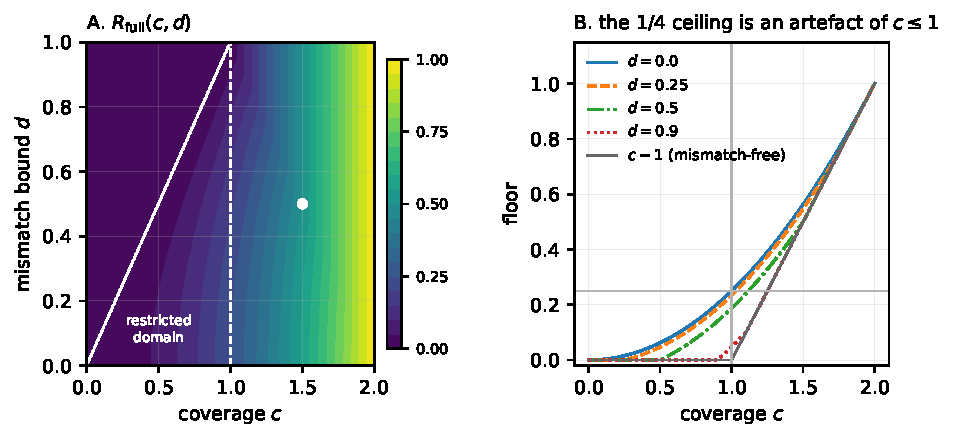
\includegraphics[width=\linewidth]{figures/floor_range.pdf}
\caption{The sharp coverage floor on the full range. \textbf{A.} $\Rfull(c,d)$
for $0\le c\le2$; the dashed box is the domain of the restricted theorem and the
white curve is the zero-floor boundary $d=c$, which exists only for $c\le1$. The
marked point is the planning row $(c,d)=(1.5,0.5)$ of
Table~\ref{tab:example}. \textbf{B.} Sections at fixed $d$, with the
mismatch-free envelope $c-1$ of Corollary~\ref{cor:highcov}; the horizontal line
is the value $1/4$ discussed in Remark~\ref{rem:ceiling}. These are exact theory
curves, not fitted data.}
\label{fig:floor}
\end{figure}

\section{The exact allocation profile}\label{sec:profile}

Theorem~\ref{thm:coverage} shows that equal allocation is maximin, but not by
how much other allocations lose, nor whether the optimum is unique. Both matter
in practice: a design that must depart from a balanced split needs the exact
price, and a numerical search over a grid cannot distinguish a unique optimum
from a plateau. We compute the profile exactly.

For $w\in[0,1]$ write $A=|2w-1|$ and let
\begin{equation}\label{eq:profile}
M(w;c,d)=
\begin{cases}
\dfrac{c^2-t^2-A^2c^2}{4}, & Ac\le \hc-t,\\[8pt]
\dfrac{c^2+\hc^2-2\hc t-2Ac(\hc-t)}{4}, & \hc-t\le Ac\le \hc,\\[8pt]
\dfrac{c^2+\hc^2-2Ac\,\hc}{4}, & Ac\ge \hc.
\end{cases}
\end{equation}
The three expressions agree on the overlaps, so $M$ is continuous, and it is
nonincreasing in $A$.

\begin{theorem}[Allocation profile]\label{thm:profile}
For $0\le c\le2$, $d\ge0$ and $w\in[0,1]$,
\[
\min_{(x,y,a,b)\in\mathcal A(c,d)}\Bigl\{w\,xy+(1-w)\,ab\Bigr\}=M(w;c,d),
\]
and the minimum is attained. In particular $M(1/2;c,d)=\Rfull(c,d)$.
\end{theorem}

\begin{proof}
\emph{Reduction.} Let $\ell,u,X,Y$ be as in the proof of
Theorem~\ref{thm:coverage}. As shown there, $xy\ge XY$ and $ab\ge(c-X)(c-Y)$
with all factors nonnegative, and $w,1-w\ge0$, so
\[
w\,xy+(1-w)\,ab\ \ge\ w\,XY+(1-w)(c-X)(c-Y),
\]
with $X,Y\in[\ell,u]$ and $|X-Y|\le t$. Conversely, for any $X,Y\in[\ell,u]$
with $|X-Y|\le d$ the quadruple $(X,Y,c-X,c-Y)$ lies in $\mathcal A(c,d)$,
because $c-X,c-Y\in[c-u,c-\ell]=[\ell,u]\subseteq[0,1]$. Hence the minimum
equals
\[
\min\Bigl\{w\,XY+(1-w)(c-X)(c-Y):\ X,Y\in[\ell,u],\ |X-Y|\le d\Bigr\}.
\]

\emph{Coordinates.} Put $\sigma=X+Y-c$ and $\tau=X-Y$. Since $\ell+u=c$ and
$u-\ell=\hc$, the constraint $X,Y\in[\ell,u]$ is exactly
$|\sigma|+|\tau|\le \hc$, and the mismatch constraint is $|\tau|\le d$; together,
$|\tau|\le\min\{d,\hc-|\sigma|\}$. A direct computation gives
\begin{equation}\label{eq:sigmatau}
w\,XY+(1-w)(c-X)(c-Y)
=\frac{\sigma^2+c^2-\tau^2+2(2w-1)c\,\sigma}{4}.
\end{equation}
Minimising over the sign of $\sigma$ replaces $2(2w-1)c\sigma$ by $-2Acv$ with
$v=|\sigma|\in[0,\hc]$, and minimising over $\tau$ takes
$|\tau|=\min\{t,\hc-v\}$. So the problem reduces to minimising
\[
f(v)=v^2+c^2-\min\{t,\hc-v\}^2-2Acv,\qquad v\in[0,\hc],
\]
and the minimum of \eqref{eq:sigmatau} is $\min_v f(v)/4$.

\emph{The one-dimensional minimisation.} On $[0,\hc-t]$ we have
$f(v)=v^2+c^2-t^2-2Acv$, a convex parabola minimised at $v=Ac$. On $[\hc-t,\hc]$
we have $f(v)=c^2-\hc^2+2v(\hc-Ac)$, which is affine in $v$ and whose value at
$v=\hc-t$ agrees with the first branch. Three cases:
if $Ac\le \hc-t$, the minimum is at $v=Ac$, with value $c^2-t^2-A^2c^2$;
if $\hc-t\le Ac\le \hc$, the first branch decreases on $[0,\hc-t]$ and the
second is nondecreasing, so the minimum is at $v=\hc-t$, with value
$c^2+\hc^2-2\hc t-2Ac(\hc-t)$;
if $Ac\ge \hc$, the second branch is nonincreasing, so the minimum is at
$v=\hc$, where $\tau=0$, with value $c^2+\hc^2-2Ac\hc$.
These are the three lines of \eqref{eq:profile}.

\emph{Attainment.} Each case exhibits an explicit minimiser $(v,|\tau|)$, namely
$(Ac,t)$, $(\hc-t,t)$ and $(\hc,0)$, all satisfying $v+|\tau|\le \hc$. Choosing
the sign of $\sigma$ opposite to that of $2w-1$ and setting
$X=(c+\sigma+\tau)/2$, $Y=(c+\sigma-\tau)/2$, $a=c-X$, $b=c-Y$ gives an
admissible source attaining the value. Finally, at $w=1/2$ we have $A=0\le
\hc-t$, and the first branch gives $(c^2-t^2)/4=\Rfull(c,d)$.
\end{proof}

\begin{corollary}[Strict loss away from balance]\label{cor:strict}
Let $0<c\le2$ and suppose the mismatch budget binds, $t<\hc$. Then
$M(w;c,d)<\Rfull(c,d)$ for every $w\ne1/2$, so equal allocation is the unique
maximin allocation.
\end{corollary}

\begin{proof}
Write $\Delta=\Rfull(c,d)-M(w;c,d)$ and $A=|2w-1|>0$, so $Ac>0$. In the first
branch $4\Delta=A^2c^2>0$. In the second branch
$4\Delta=(\hc-t)\bigl(2Ac-(\hc-t)\bigr)>0$, because $\hc-t>0$ and
$2Ac>\hc-t$ by the branch condition. In the third branch
$4\Delta=2Ac\,\hc-\hc^2-t^2\ge2\hc^2-\hc^2-t^2=\hc^2-t^2>0$, again by the
branch condition.
\end{proof}

\begin{corollary}[Plateau when the budget does not bind]\label{cor:plateau}
If $\hc\le d$, so that $t=\hc$, then $M(w;c,d)=\Rfull(c,d)$ for every $w$ with
$|2w-1|\,c\le \hc$, and $M$ is strictly decreasing in $A$ beyond that point. For
$c\le1$ this plateau is the whole interval $w\in[0,1]$ at the value $0$; for
$c>1$ it is an interval of half-width $(2-c)/(2c)$ around $w=1/2$ at the
positive value $(c^2-(2-c)^2)/4=c-1$.
\end{corollary}

\begin{proof}
With $t=\hc$ the first branch applies only at $A=0$ and the second branch gives
$\bigl(c^2+\hc^2-2\hc^2-0\bigr)/4=(c^2-\hc^2)/4=\Rfull(c,d)$ on the whole range
$Ac\le \hc$. Beyond it the third branch is strictly decreasing in $A$ when
$\hc>0$.
\end{proof}

Corollary~\ref{cor:plateau} is the honest reading of an earlier numerical
observation that a grid search over $w$ failed to select $w=1/2$: on a
non-binding mismatch budget there is nothing to select, because a whole interval
of allocations is optimal. Figure~\ref{fig:alloc} plots both regimes together
with brute-force minima computed independently of \eqref{eq:profile}.

\begin{figure}[ht]
\centering
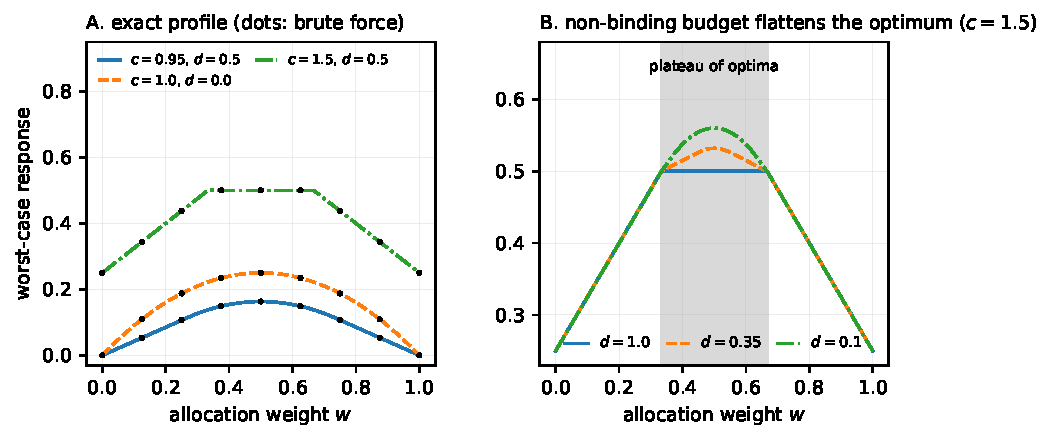
\includegraphics[width=\linewidth]{figures/allocation.pdf}
\caption{Worst-case response as a function of the allocation weight.
\textbf{A.} Exact profile \eqref{eq:profile} (curves) against an independent
brute-force minimisation over the admissible source set (dots); the kinks are
the branch boundaries of Theorem~\ref{thm:profile}. \textbf{B.} A non-binding
mismatch budget produces a plateau of optima (shaded), of half-width
$(2-c)/(2c)$ in $w$, as in Corollary~\ref{cor:plateau}. All curves are exact
theory.}
\label{fig:alloc}
\end{figure}

\section{Mismatch in mean square}\label{sec:moment}

A uniform per-type bound $|x_z-y_z|\le d$ is a strong calibration requirement:
it must hold for every recoverable type, including types that are rare. The next
result shows that only a population average is needed, with the same floor.

\begin{theorem}[Mean-square mismatch]\label{thm:moment}
Let $\mu$ be a probability weight on recoverable types, let every type satisfy
the coverage constraints $x_z+a_z\ge c$ and $y_z+b_z\ge c$ with
$x_z,y_z,a_z,b_z\in[0,1]$ and $0\le c\le2$, and suppose
\[
\E_\mu\bigl[(x-y)^2\bigr]=\sum_z\mu_z(x_z-y_z)^2\le D^2,\qquad D\ge0 .
\]
Then
\[
\E_\mu\Bigl[\frac{xy+ab}{2}\Bigr]\ \ge\ \Rfull(c,D),
\]
and the bound is attained by the constant type \eqref{eq:witness} with
$t=\min\{D,\hc\}$. The uniform-mismatch case of Theorem~\ref{thm:coverage} is
the special case $D=d$.
\end{theorem}

\begin{proof}
Apply the lower bound \eqref{eq:identity} to each type with its own mismatch,
which gives, with $t_z=\min\{|x_z-y_z|,\hc\}$,
\[
\frac{x_zy_z+a_zb_z}{2}\ \ge\ \frac{c^2-t_z^2}{4}.
\]
Averaging, $\E_\mu[(xy+ab)/2]\ge(c^2-\E_\mu[t^2])/4$. Now
$t_z^2\le(x_z-y_z)^2$ and $t_z^2\le \hc^2$ pointwise, so
$\E_\mu[t^2]\le\min\{D^2,\hc^2\}=\min\{D,\hc\}^2$, which is the claim. The
constant type \eqref{eq:witness} with $t=\min\{D,\hc\}$ has mean-square mismatch
exactly $t^2\le D^2$ and attains the value. A uniform bound $|x_z-y_z|\le d$
implies $\E_\mu[(x-y)^2]\le d^2$, giving the stated special case.
\end{proof}

Theorem~\ref{thm:moment} is genuinely weaker as a hypothesis: a small population
of badly mismatched types is tolerated provided the mean square stays within
budget. What cannot be weakened is the requirement that the average be taken
over the \emph{recoverable} population with its own weights. Two pooled
summaries that look similar are not sufficient.

\begin{example}[Equal stage means do not suffice]\label{ex:means}
Let two types have weight $1/2$ each, with $(x,y)=(1,0)$ and $(x,y)=(0,1)$, and
exactly complementary partners. Then $\E[x]=\E[y]=1/2$, yet $\E[xy]=0$ and the
complementary complete paths also vanish, so the average complete-path response
is $0$. The mean-square mismatch is $1$, and Theorem~\ref{thm:moment} correctly
returns $\Rfull(1,1)=0$. Equality of the two stage means carries no information
about their joint behaviour within a type.
\end{example}

\begin{example}[The pooled conditional is not the mean second stage]\label{ex:pooled}
For the mixture of Example~\ref{ex:means}, the pooled second-stage conditional
probability is
\[
\Prob(D_1\mid A_1)=\frac{\E[xy]}{\E[x]}=0\neq\frac12=\E[y],
\]
whenever $\E[x]>0$. Averaging conditional probabilities across latent types
without activation weights can manufacture an apparent alignment that the source
does not possess. A calibration that reports $\E[x]$ and $\E[y]$ separately does
not bound $d$ or $D$.
\end{example}

\section{From source paths to a finite negative certificate}\label{sec:certificate}

We now compose the source floor with recording losses, exceptional types, an
explicit sampling law and a calibration allowance.

\subsection{Recorded response of a heterogeneous population}

Let a covered subset of recoverable types carry mass at least $1-\eta$. Only
covered types must satisfy the coverage constraints, with conditional mismatch
budget $D$ in the sense of Theorem~\ref{thm:moment}; their completed paths are
recorded with conditional probabilities $r_z,s_z\ge\kappa$. All remaining
contributions may be zero. Define the recorded per-condition responses
\begin{equation}\label{eq:uv}
u=\sum_z\mu_zx_zy_zr_z,\qquad v=\sum_z\mu_za_zb_zs_z .
\end{equation}

\begin{proposition}[Recording and exceptional mass]\label{prop:record}
Under these assumptions,
\begin{equation}\label{eq:g}
\frac{u+v}{2}\ \ge\ g:=(1-\eta)\,\kappa\,\Rfull(c,D),
\end{equation}
and the bound is sharp in the class that admits invisible exceptional types and
recording probability exactly $\kappa$ on covered paths.
\end{proposition}

\begin{proof}
On each covered type, nonnegativity of the path probabilities and $r_z,s_z\ge
\kappa$ give $(x_zy_zr_z+a_zb_zs_z)/2\ge\kappa(x_zy_z+a_zb_z)/2$. Summing over
covered types and applying Theorem~\ref{thm:moment} to the covered submixture,
whose total mass $m\ge1-\eta$, yields
$\sum_{\text{covered}}\mu_z(x_zy_zr_z+a_zb_zs_z)/2\ge\kappa\,m\,\Rfull(c,D)\ge
\kappa(1-\eta)\Rfull(c,D)$, using $\Rfull\ge0$. Discarding the nonnegative
contributions of exceptional types gives \eqref{eq:g}. For sharpness, place mass
$1-\eta$ on the attaining type \eqref{eq:witness}, set both recording
probabilities to $\kappa$, and place mass $\eta$ on a type with $x=y=a=b=0$;
then $u=v=g$.
\end{proof}

No independence of recording and phenotype is used: the recording bound is
stated conditionally on the completed path and the type. A product of a
retention bound and an instrumental detection bound is legitimate only if each
applies conditionally at its own stage; two marginal success rates do not
automatically justify their product. The interpretation of $\eta$ is equally
strict: it bounds uncovered mass among true reference-recoverable units, not the
share of unusual types among observed positives.

\subsection{The observation law is derived, not postulated}

\begin{lemma}[Terminal masses and the all-negative event]\label{lem:likelihood}
Fix a condition and a type with stage probabilities $(x,y)$ and recording
probability $r$. The five terminal source events of Figure~\ref{fig:paths} carry
masses
\begin{equation}\label{eq:paths}
1-p,\qquad p(1-x),\qquad px(1-y),\qquad pxy(1-r),\qquad pxyr,
\end{equation}
which are nonnegative and sum to one; the first four, which are exactly the
negative records, sum to $1-pxyr$. Mixing over types, a unit in condition~1 is
negative with probability $1-pu$ and a unit in condition~2 with probability
$1-pv$. For $n=2m$ independent units with $m$ assigned to each condition
independently of type,
\begin{equation}\label{eq:allneg}
\Prob(\text{all negative})=(1-pu)^m(1-pv)^m .
\end{equation}
\end{lemma}

\begin{proof}
Nonnegativity and normalisation of \eqref{eq:paths} are immediate, and the first
four entries sum to $1-pxyr$. Averaging over the type weights gives $1-pu$ and
$1-pv$ by \eqref{eq:uv}. Independent units have product masses over histories;
summing those products over all histories in which every unit is negative
factors into \eqref{eq:allneg}.
\end{proof}

Equation \eqref{eq:allneg} is a consequence of the source events, not an extra
modelling assumption about wells. This matters, because it is precisely the step
at which an unjustified independence or an unnoticed change of denominator would
enter.

\subsection{Balanced design and conditional calibration}

\begin{theorem}[Balanced sampling with a calibration allowance]\label{thm:root}
Take $n=2m$ independent eligible units from the common source, $m$ per
condition. Suppose that on every \emph{good} calibration environment the source
and recording contract of Proposition~\ref{prop:record} holds with fixed
$c,D,\kappa,\eta$, and that the probability of a bad environment is at most
$\delta\in[0,1]$. Then for $0<\theta\le p\le1$ the rule that certifies
$p<\theta$ exactly on an all-confirmed-negative record has false-certification
probability at most
\begin{equation}\label{eq:root}
\delta+(1-\delta)\,(1-\theta g)^n,\qquad g=(1-\eta)\kappa\Rfull(c,D).
\end{equation}
The bound is attained in the stated class, by the mixture of
Proposition~\ref{prop:record} with $p=\theta$, bad mass exactly $\delta$, and bad
environments that certify with probability one.
\end{theorem}

\begin{proof}
Condition on a good environment and use Lemma~\ref{lem:likelihood}. All bases are
nonnegative, since $pu,pv\le1$. The identity
\begin{equation}\label{eq:amgm}
\Bigl(1-p\frac{u+v}{2}\Bigr)^2-(1-pu)(1-pv)=\frac{p^2(u-v)^2}{4}\ \ge\ 0
\end{equation}
gives $(1-pu)^m(1-pv)^m\le\bigl(1-p(u+v)/2\bigr)^{2m}$, and
$p\ge\theta$ with \eqref{eq:g} gives
$\bigl(1-p(u+v)/2\bigr)^{n}\le(1-\theta g)^n=:B$. If the actual bad mass is
$\beta\le\delta$, the total false-certificate probability is at most
$(1-\beta)B+\beta\le(1-\delta)B+\delta$, because $B\le1$. Attainment: the
mixture of Proposition~\ref{prop:record} has $u=v=g$, so with $p=\theta$ the
conditional bound holds with equality, and equality in the composition requires
exactly the stated bad-environment behaviour.
\end{proof}

The composition does not require independence between calibration and the future
experiment. It does require the sampling guarantee to hold \emph{conditionally on
every good environment}. A marginal confidence statement about a calibration
estimate does not by itself supply that contract when data are reused, when
several bounds are selected after inspection, or when batch effects are shared;
in those cases the environment allowance $\delta$ must be constructed to cover
the selection.

\begin{remark}[Independent random allocation, and unbalanced designs]
If each unit independently receives condition~1 or~2 with probability $1/2$, its
negative mass is $1-p(u+v)/2$ and the all-negative law is
$\bigl(1-p(u+v)/2\bigr)^n$ for any integer $n$, with the same worst-case bound.
By \eqref{eq:amgm}, for a fixed response pair the balanced fixed design is no
worse than random assignment at even $n$. An unbalanced fixed design instead has
$(1-pu)^{n_1}(1-pv)^{n_2}$; substituting an observed allocation fraction into
the random-assignment formula does not reproduce that law.
\end{remark}

\section{Sample size, feasibility and reporting}\label{sec:sample}

Assume $0\le\delta<\alpha<1$, $0<\theta\le1$ and $g>0$, and set
\begin{equation}\label{eq:Bstar}
B_*=\frac{\alpha-\delta}{1-\delta},\qquad z=\theta g\in(0,1] .
\end{equation}
The bound \eqref{eq:root} is at most $\alpha$ exactly when $(1-z)^n\le B_*$. For
$z<1$, taking logarithms gives the random-assignment minimum
\begin{equation}\label{eq:nmin}
n_{\min}=\left\lceil\frac{\log B_*}{\log(1-z)}\right\rceil,
\end{equation}
and for a fixed balanced design one takes the smallest even integer at least
$n_{\min}$. These are minima within the stated design class and for the stated
all-negative rule; they are not claims about every possible observation
technology, and a rule that never certifies trivially has zero false-certificate
probability while performing no task. Writing $H=\log(1/B_*)$ and integrating
$1/(1-s)$ on $[0,z]$ gives $z\le-\log(1-z)\le z/(1-z)$, hence the unrounded
requirement $n_*$ obeys
\begin{equation}\label{eq:sandwich}
\frac{H(1-z)}{z}\ \le\ n_*\ \le\ \frac Hz .
\end{equation}
The simple bound $\lceil H/z\rceil$, rounded up to an even integer, is always
sufficient.

On the restricted range $g\le1/4$, so $z<1$ automatically and \eqref{eq:nmin}
always applies. On the full range $g$ can reach $1$ --- at $c=2$, $\kappa=1$,
$\eta=0$ --- and then $z=\theta g$ can equal $1$, in which case a single unit
already has zero good-environment negative probability. The feasibility boundary
must therefore be stated with that case separated.

\begin{theorem}[Exact finite feasibility]\label{thm:feasible}
Let $0\le z\le1$, $0\le\delta\le1$ and $0<\alpha<1$. There exists an integer
$m\ge1$ with $\delta+(1-\delta)(1-z)^{2m}\le\alpha$ if and only if
\[
\bigl(z>0\ \text{and}\ \delta<\alpha\bigr)\quad\text{or}\quad
\bigl(z=1\ \text{and}\ \delta\le\alpha\bigr).
\]
\end{theorem}

\begin{proof}
($\Rightarrow$) Suppose $m\ge1$ satisfies the bound. Since $\delta\le1$ and
$(1-z)^{2m}\ge0$, the added term is nonnegative, so $\delta\le\alpha<1$ and
hence $1-\delta>0$. If $z=0$ the left-hand side is $\delta+(1-\delta)=1>\alpha$,
so $z>0$. If moreover $\delta\ge\alpha$, then
$(1-\delta)(1-z)^{2m}\le\alpha-\delta\le0$, and $1-\delta>0$ with
$(1-z)^{2m}\ge0$ forces $(1-z)^{2m}=0$, hence $z=1$; the displayed bound then
reads $\delta\le\alpha$.

($\Leftarrow$) If $z=1$ take $m=1$: the error is $\delta\le\alpha$. If $z>0$ and
$\delta<\alpha$, then $0\le1-z<1$, so there is $k$ with
$(1-z)^k<\alpha-\delta$. Take $m=k+1$, so $2m\ge k$ and hence
$(1-z)^{2m}\le(1-z)^k$; since $0\le1-\delta\le1$,
$\delta+(1-\delta)(1-z)^{2m}\le\delta+(1-z)^k<\alpha$.
\end{proof}

\begin{corollary}[Feasibility in terms of the source parameters]\label{cor:feasible}
With $g=(1-\eta)\kappa\Rfull(c,D)$ and $0<\alpha<1$, a finite balanced sample
attains uniform total error at most $\alpha$ over the full sharpness class if and
only if $\theta>0$, $\kappa>0$, $\eta<1$, $\Rfull(c,D)>0$ and $\delta<\alpha$,
or else $\theta g=1$ and $\delta\le\alpha$. Moreover $\Rfull(c,D)>0$ holds
exactly when $c>0$ and $\min\{D,\hc\}<c$; on the restricted range this is
$c>D$, while for $c>1$ it is automatic.
\end{corollary}

\begin{proof}
Combine Theorem~\ref{thm:feasible} with $z=\theta g$ and the positivity
statements: $g>0$ iff each factor is positive, and $\Rfull(c,D)=(c^2-t^2)/4>0$
iff $t<c$, where $t=\min\{D,\hc\}\le \hc$. For $c>1$, $\hc=2-c<c$, so $t<c$
always; for $c\le1$, $\hc=c$ and $t<c$ iff $D<c$.
\end{proof}

This is a statement about a \emph{uniform guarantee over a model class}. A real
assay may perform well when the available bounds are too weak to certify it;
failure of the sufficient information is not evidence of biological failure.

\begin{proposition}[All-negative confidence endpoint]\label{prop:endpoint}
For $n>0$ and $g>0$ define, on an evaluable all-negative record,
\begin{equation}\label{eq:upper}
p_U=\min\Bigl\{1,\ \frac{1-B_*^{1/n}}{g}\Bigr\},
\end{equation}
and return the endpoint $1$ on every other record. Then the interval $[0,p_U]$
has coverage at least $1-\alpha$ for the true recoverable fraction.
\end{proposition}

\begin{proof}
Coverage can fail only on an all-negative record with $p>p_U$, which requires
$p_U<1$ and hence $pg>1-B_*^{1/n}$, that is $(1-pg)^n<B_*$. By
Theorem~\ref{thm:root} applied with $\theta=p$, the probability of that record is
at most $\delta+(1-\delta)(1-pg)^n<\delta+(1-\delta)B_*=\alpha$.
\end{proof}

This is a deliberately limited procedure: positive or unevaluable records return
an uninformative endpoint rather than an unsupported point estimate, and the
statement concerns repeated sampling, not the posterior probability that a
particular specimen is sterile. For computation use
$p_U=-\mathrm{expm1}\bigl(\log(B_*)/n\bigr)/g$, capped at one, which avoids
cancellation when the root is close to one; if $g=0$, $n=0$ or $\delta\ge\alpha$,
report the certificate as unavailable rather than evaluating \eqref{eq:upper}.

\begin{proposition}[Cost of a closing margin]\label{prop:asym}
As $z\to0$, $n_*=H\bigl(1/z-1/2+O(z)\bigr)$. With $\theta,\kappa,1-\eta$ fixed
and positive and $0<c\le1$, the requirement diverges as the coverage margin
closes:
\[
n_*\ \sim\ \frac{2H}{\theta(1-\eta)\kappa\,c\,(c-D)}\qquad (D\uparrow c),
\]
and in the rare-detection regime
$\partial\log n_*/\partial c\approx-2c/(c^2-D^2)$ and
$\partial\log n_*/\partial D\approx 2D/(c^2-D^2)$. Integer rounding changes $n_*$
by a bounded additive amount. As $\delta\uparrow\alpha$, $H\to\infty$: no
increase in the number of units crosses the calibration-failure boundary.
\end{proposition}

\begin{proof}
Expand $-\log(1-z)=z+z^2/2+O(z^3)$ in $n_*=H/(-\log(1-z))$. With
$\Rfull(c,D)=(c-D)(c+D)/4$ on the restricted range and $D\uparrow c$,
$z=\theta(1-\eta)\kappa(c-D)(c+D)/4\sim\theta(1-\eta)\kappa c(c-D)/2$, and
$n_*\sim H/z$. The derivatives follow from $n_*\approx4H/[\theta(1-\eta)\kappa
(c^2-D^2)]$, and $H=\log\bigl((1-\delta)/(\alpha-\delta)\bigr)\to\infty$ as
$\delta\uparrow\alpha$.
\end{proof}

\section{Adaptive reallocation does not help}\label{sec:adaptive}

Theorem~\ref{thm:coverage} assumes the allocation is fixed in advance. A natural
question is whether choosing each unit's condition in the light of previous
outcomes improves the guarantee. It does not.

\begin{theorem}[Adaptive policies face the same bound]\label{thm:adaptive}
Consider a budget of $n$ fresh independent units. A policy may choose the
condition of each unit as a (possibly randomized) function of the outcomes of the
previously observed units, but cannot change a unit's condition after observing
its own stage trajectory; the qualifying event is the same in both conditions and
the certificate is issued exactly on an all-negative record. Then for every such
policy the worst-case false-certificate probability over the class of
Theorem~\ref{thm:root} is at least $\delta+(1-\delta)(1-\theta g)^n$, which the
fixed balanced design attains.
\end{theorem}

\begin{proof}
Evaluate the policy on the attaining population of
Proposition~\ref{prop:record}, which has recorded response $u=v=g$ in
\emph{both} conditions, with $p=\theta$. Let $N_i$ be the event that the first
$i$ units are negative. Conditional on $N_{i-1}$ and on the policy's choice for
unit $i$ --- which is measurable with respect to the first $i-1$ outcomes and
independent randomisation --- unit $i$ is recorded positive with probability
$\theta u=\theta v=\theta g$, since the unit is fresh and independent of the
past. Hence $\Prob(N_i\mid N_{i-1})=1-\theta g$ whatever the choice, and
$\Prob(N_n)=(1-\theta g)^n$ by the chain rule. Adding bad environments of mass
$\delta$ that certify with probability one gives the stated value, and
Theorem~\ref{thm:root} shows the balanced design attains it.
\end{proof}

The scope of Theorem~\ref{thm:adaptive} should be read carefully. Adaptivity may
well improve performance on populations other than the least detectable one; and
the result says nothing about designs that switch conditions \emph{within} a
unit, introduce a new readout, change the reference task, or decline to certify
some all-negative records. Switching within a unit is a genuinely different
causal question, discussed in Section~\ref{sec:limits}.

\section{A reproducible synthetic planning example}\label{sec:example}

Table~\ref{tab:example} fixes $\theta=0.01$, $\alpha=0.05$, the exposure and the
observation deadline. Every parameter is synthetic; no row is an estimated
operating characteristic of any assay. The rows successively relax ideal
coverage, allow recording loss and an exceptional recoverable fraction, allocate
error to calibration failure, and finally exploit the full coverage range.

\begin{table}[ht]
\centering\small
\begin{tabularx}{\linewidth}{@{}Y r r r r@{}}
\toprule
Planning assumptions & $g$ & $n_{\min}$ & Balanced $n$ & Total error\\
\midrule
\planningrows
\bottomrule
\end{tabularx}
\caption{Exact integer planning checks; displayed probabilities are rounded.
Unspecified factors are ideal and $\delta=0$ except where stated. The column
$n_{\min}$ uses independent random assignment and the next column is the
smallest even sample for the fixed balanced theorem. The last row uses
$c=1.5$ with $\kappa=.90$, $\eta=.05$, $\delta=.01$, and is licensed only by
Theorem~\ref{thm:coverage} on the full range.}
\label{tab:example}
\end{table}

In the fourth row, $\Rfull=261/1600$, $g=44631/320000$ and $B_*=4/99$, and the
integer threshold is confirmed by exact rational arithmetic:
\begin{equation}\label{eq:exact}
\Bigl(1-\frac{44631}{32000000}\Bigr)^{2300}\le\frac4{99}
<\Bigl(1-\frac{44631}{32000000}\Bigr)^{2299},
\end{equation}
the corresponding total errors being $0.0499494$ and $0.0500052$; so $2299$
units narrowly fail the budget and $2300$ succeed. The all-negative endpoint
\eqref{eq:upper} at $n=2300$ is $p_U\approx0.0099961$. In the last row,
$\Rfull(1.5,0.5)=1/2$ and $g=171/400=0.4275$, giving $749$ and $750$ units at
total error $0.0498285$: a factor of about three fewer units than the fourth
row, obtained entirely by strengthening the coverage premise beyond $c=1$. On the
restricted range no premise whatever can beat $g\le1/4$.

The earlier compiled regression of this model uses $\theta=1/5$, $c=1$, $d=1/2$
and $n=100$, with $(1-\theta R)^{100}=(77/80)^{100}\approx0.0218813<0.05$; its
exact minima are $79$ units under random assignment and $80$ under a balanced
design, so the $100$-unit example is valid but deliberately conservative.

Figure~\ref{fig:design} shows why the margin, rather than the number of units,
dominates feasibility. Its curves use the unrounded requirement; the table gives
integer designs. A permissible report would read:

\begin{quote}
``All $2{,}300$ eligible tracked units had no qualifying recorded event. Under
the stated recovery-coverage, exceptional-mass, recording and calibration
assumptions, this procedure excludes a reference-recoverable fraction of $1\%$
or more with false-certificate probability at most $5\%$.''
\end{quote}

The eligible denominator must be stated explicitly. If eligibility selects intact
cells found after exposure, the fraction refers to that selected population; it
does not directly quantify killing among the originally exposed cells.

\begin{figure}[ht]
\centering
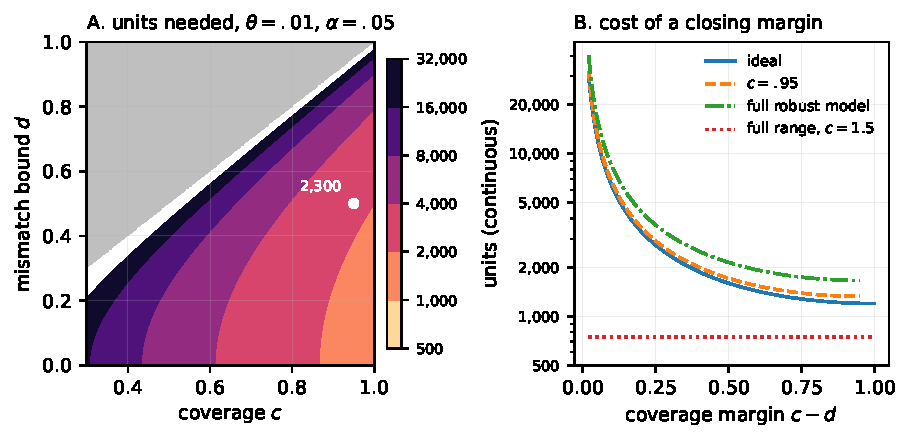
\includegraphics[width=\linewidth]{figures/design.pdf}
\caption{Synthetic design consequences. \textbf{A.} Units required on the
restricted range for $\theta=.01$, $\alpha=.05$, $\kappa=.90$, $\eta=.05$,
$\delta=.01$; the grey region has no positive uniform floor and the marked point
is the fourth row of Table~\ref{tab:example}. \textbf{B.} Cost of a closing
coverage margin $c-D$ on a logarithmic scale, including the full-range row with
$c=1.5$. These are exact theory curves, not fitted data or Monte Carlo
estimates.}
\label{fig:design}
\end{figure}

\section{What must be established experimentally}\label{sec:limits}

The decisive unresolved question is empirical: whether an exposed target
population and a paired recovery design support the joint bounds of
Table~\ref{tab:calibration}. Neither random assignment alone nor pooled stage
means identify within-type potential responses in two conditions, and a single
unit generally cannot undergo both potential recovery histories. Mechanistic
transport, replicate lineages or calibrated strata can supply the missing
information only with their own explicit assumptions.

\begin{table}[ht]
\centering\small
\begin{tabularx}{\linewidth}{@{}l Y Y@{}}
\toprule
Premise & Required information & Insufficient substitute\\
\midrule
Reference task & Defined recoverability endpoint and target population &
Calling every finite non-crosser dead\\
$c$ & Stage coverage across conditions, transported to exposed types &
High response in an unrelated healthy control\\
$d$ or $D$ & Joint type-level stage information, or a structural bound &
Equal marginal stage means (Examples~\ref{ex:means},~\ref{ex:pooled})\\
$\eta$ & Uncovered mass among reference-recoverable types &
Unusual-type fraction among observed positives\\
$\kappa$ & Recording bound conditional on completed paths and phenotype &
Pooled instrumental accuracy\\
$\delta$ & Simultaneous calibration and a conditional future-experiment contract &
Unadjusted marginal intervals or adaptive data reuse\\
Independent units & Sampling, assignment, batch and lineage provenance &
Counting images or descendants as new replicates\\
\bottomrule
\end{tabularx}
\caption{The mathematical assumptions define an empirical validation task. They
are not established by the theorems or by the synthetic example, and the numbers
$c$, $d$ and $D$ are properties of a declared event model and population, not
universal physiological constants.}
\label{tab:calibration}
\end{table}

\paragraph{Shared failures are not independent recording losses.}
If an entire run fails with probability $\rho$, the negative probability can be
$\rho+(1-\rho)(1-pg)^n$. The floor $\rho$ does not shrink by adding units to the
same failing run; independent batches may help under a separate, justified batch
model. The calibration allowance $\delta$ and a physical shared failure $\rho$
should not be equated or added without specifying their relationship.

\paragraph{Losses must not be silently dropped.}
One safe rule certifies only when every required record is evaluable and
negative, which shrinks the certification event and preserves the bound.
Alternatively, losses can enter a justified conditional recording model.
Discarding lost units and recomputing an apparently clean denominator requires a
new sampling argument.

\paragraph{A recovery certificate is not a killing curve.}
For two exposures with comparable original denominators, write the observable
event fractions as $r_0=p_0g_0$ and $r_\tau=p_\tau g_\tau$. Then
\begin{equation}\label{eq:ratio}
\frac{p_\tau}{p_0}=\frac{r_\tau}{r_0}\cdot\frac{g_0}{g_\tau},
\end{equation}
so a tenfold decrease in recorded events is equally consistent with a tenfold
decrease in recovery sensitivity: $p_\tau=p_0$ with $g_0=0.8$ and $g_\tau=0.08$
produces it. If separately justified bounds $g_j\in[L_j,U_j]$ are available, then
$\frac{r_\tau}{r_0}\frac{L_0}{U_\tau}\le\frac{p_\tau}{p_0}\le
\frac{r_\tau}{r_0}\frac{U_0}{L_\tau}$, and finite-sample uncertainty in
$r_0,r_\tau$ must be propagated in addition. Equation \eqref{eq:ratio} is
algebra, not a new estimator; it explains why a recovery certificate and a
quantitative killing curve \citep{brauner2017} require related but distinct
calibration tasks.

\paragraph{Stage switching is a separate causal question.}
If the condition could be randomized independently at each stage and the stage
probabilities transported unchanged across switches, then in the exactly
complementary model the four schedules average to
$\bigl(xy+x(1-y)+(1-x)y+(1-x)(1-y)\bigr)/4=1/4$, bypassing the mismatch
obstruction entirely. But the unswitched observations identify only two of the
four paths; cross-condition stage behaviour may differ, and with unconstrained
cross responses switching need not help. This is a precisely stated future
intervention hypothesis, not a laboratory recommendation: its missing premise is
the behaviour of the activated state under a changed condition.

\paragraph{A shortcut when direct calibration is available.}
If independently ascertained reference-positive units provide a representative
direct lower bound on the average recorded recovery $g$, the sampling results of
Section~\ref{sec:certificate} apply to that bound directly and the two-stage
model is a diagnostic explanation rather than a mandatory calibration ritual.
The ascertainment must not exclude the slow or difficult units the claim intends
to cover; reference-positive units selected because the test already detected
them make the argument circular.

\section{Formal verification and reproducibility}\label{sec:formal}

The source is represented by normalized nonnegative finite path weights and
independence by products over finite histories; the decision chain is therefore
finite and elementary, and is machine-checkable end to end. Table~\ref{tab:formal}
maps each result of this paper to its status.

\begin{table}[ht]
\centering\footnotesize
\begin{tabularx}{\linewidth}{@{}>{\raggedright\arraybackslash}p{4.4cm} l Y@{}}
\toprule
Result & Status & Lean declaration (namespace \leanref{FunctionalViability.Robust})\\
\midrule
Theorem~\ref{thm:coverage}, bound & compiled & \leanref{extended\_\allowbreak{}coverage\_\allowbreak{}bound}\\
Theorem~\ref{thm:coverage}, witness and maximin & compiled &
\leanref{extended\_\allowbreak{}sharp\_\allowbreak{}witness}, \leanref{extended\_\allowbreak{}minimax}\\
Corollary~\ref{cor:restricted} & compiled & \leanref{extended\_\allowbreak{}eq\_\allowbreak{}recoveryFloor}\\
Corollary~\ref{cor:highcov} & compiled & \leanref{extended\_\allowbreak{}high\_\allowbreak{}coverage}\\
Corollary~\ref{cor:approx} & compiled & \leanref{approximate\_\allowbreak{}complementarity},
\leanref{approximate\_\allowbreak{}complementarity\_\allowbreak{}sharp}\\
Theorem~\ref{thm:profile} & compiled & \leanref{allocation\_\allowbreak{}profile}
(\leanref{allocation\_\allowbreak{}lower}, \leanref{allocation\_\allowbreak{}attained})\\
Corollaries~\ref{cor:strict},~\ref{cor:plateau} & compiled &
\leanref{allocation\_\allowbreak{}strict}, \leanref{allocation\_\allowbreak{}plateau},
\leanref{allocation\_\allowbreak{}half}\\
Theorem~\ref{thm:moment} and Proposition~\ref{prop:record}, bound & compiled &
\leanref{moment\_\allowbreak{}population\_\allowbreak{}floor}\\
Lemma~\ref{lem:likelihood} & compiled & \leanref{stage\_\allowbreak{}normalized},
\leanref{stage\_\allowbreak{}negative}, \leanref{balanced\_\allowbreak{}identity}\\
Theorem~\ref{thm:root}, bound & compiled & \leanref{moment\_\allowbreak{}source\_\allowbreak{}certificate},
\leanref{moment\_\allowbreak{}calibrated\_\allowbreak{}certificate}\\
Theorem~\ref{thm:feasible} & compiled & \leanref{finite\_\allowbreak{}feasibility}\\
\midrule
Propositions~\ref{prop:ident},~\ref{prop:timing} & conventional &
identified set and timing rescaling\\
Sharpness constructions of
Proposition~\ref{prop:record}, Theorem~\ref{thm:root} & conventional &
exceptional mixture and bad environments\\
Equations \eqref{eq:nmin}--\eqref{eq:sandwich},
Corollary~\ref{cor:feasible} & conventional & logarithmic planning\\
Proposition~\ref{prop:endpoint}, Proposition~\ref{prop:asym} & conventional &
confidence inversion, asymptotics\\
Theorem~\ref{thm:adaptive} & conventional & adaptive-policy minimax\\
Section~\ref{sec:limits} & conventional & interpretation and algebra\\
\bottomrule
\end{tabularx}
\caption{Scope of the formal verification. ``Compiled'' means the stated
inequality or identity is proved in Lean; the biological interpretation of any
statement is never part of what a proof assistant checks.}
\label{tab:formal}
\end{table}

The environment is Lean~4.30.0 with the repository's pinned Mathlib dependency
manifest (SHA-256 \texttt{a8df0b60\ldots6e9fac}). Compilation is strict, with
warnings as errors; no proof uses \texttt{sorry} and every exported declaration
depends only on the three standard Mathlib axioms \texttt{propext},
\texttt{Classical.choice} and \texttt{Quot.sound}. The new modules are
\texttt{ExtendedCoverage.lean} (SHA-256 \texttt{3c7aef3b\ldots3c9f8a10}) and
\texttt{DesignLimits.lean} (SHA-256 \texttt{86d0340d\ldots3ef26f61}), which build
on the earlier chain \texttt{RecoverySource}, \texttt{Sampling},
\texttt{CoverageBounds}, \texttt{BalancedSampling} and \texttt{RobustCertificate}
(SHA-256 \texttt{c29773c7\ldots07d9306c6}). Verification receipts record the
compiler command, the source hash, the manifest hash, the elaborated statement
of each exported declaration and its axiom list.

A complementary script recomputes every printed constant: the exact rational
values of $\Rfull$ and $g$ in Table~\ref{tab:example}, the integer budgets with
their neighbouring powers as in \eqref{eq:exact}, the endpoint
\eqref{eq:upper}, the asymptotic ratio of Proposition~\ref{prop:asym}, and an
independent brute-force minimisation of the source problem that reproduces
$\Rfull$ and the three-branch profile \eqref{eq:profile} to $10^{-11}$ across the
full range. The figures are regenerated by the same script, so no number in the
paper is transcribed by hand.

\section{Discussion}\label{sec:discussion}

The result is conditional but operational. A justified positive coverage margin,
a recording floor, a bound on exceptional recoverable mass and a calibration
allowance yield an explicit finite error guarantee and an explicit number of
units; an admitted invisible type, a zero margin or a shared run failure
prevents it, and no amount of additional sampling repairs any of these. Three
points deserve emphasis.

First, the arithmetic of the floor is not an artefact of the restricted
parameterisation. Extending $c$ to its natural range $[0,2]$ changes the sharp
value, removes the apparent $1/4$ ceiling, produces a positive floor with no
mismatch information at all once $c>1$, and --- as the last row of
Table~\ref{tab:example} shows --- changes a planning answer by a factor of three.
Readers who encounter such a ceiling in a related model should check whether it
is a theorem or a domain convention.

Second, sharpness statements are claims about a class. Every optimum here is
attained by an explicit source, so the bounds cannot be improved without adding
a hypothesis that excludes those sources. That is a strength for design --- one
knows exactly what is being protected against --- and a limitation for
interpretation: a real population is usually not the least detectable one, so
the guarantee is conservative by construction.

Third, the mathematics cannot supply the premises. Establishing $c$, $D$,
$\kappa$, $\eta$ and $\delta$ for an exposed population, with a reference task
that is not defined circularly as ``whatever this test detects'', remains the
central empirical task. Until that is done, an all-negative record is a statement
about what was observed, not about what is alive; the viable-but-nonculturable
literature \citep{oliver2010} and the persistence literature
\citep{balaban2004,balaban2019} both suggest that the gap between the two is
where the biology lives.

\paragraph{Data and code availability.}
No new experimental data were generated or analysed. The Lean sources,
verification receipts, the numerical script that reproduces every constant and
figure, and the manuscript sources accompany this article.

\bibliographystyle{plainnat}
\bibliography{references}

\end{document}
